\documentclass[11pt]{article}

\usepackage[margin=2.3cm]{geometry}
\usepackage[T1]{fontenc}
\usepackage{lmodern}
\usepackage{amsmath,amssymb,bm}
\usepackage{booktabs}
\usepackage{xcolor}
\usepackage{tikz}
\usetikzlibrary{positioning,arrows.meta,calc,fit,backgrounds}
\usepackage{caption}
\usepackage[colorlinks=true,linkcolor=blue!50!black,citecolor=blue!50!black,urlcolor=blue!50!black]{hyperref}

\captionsetup{font=small,labelfont=bf}

\tikzset{
  box/.style={draw,rounded corners=2pt,align=center,font=\footnotesize,minimum height=7mm,inner sep=3pt,fill=white},
  inp/.style={box,fill=blue!6},
  op/.style={box,fill=gray!8},
  outputnode/.style={box,fill=green!8},
  arr/.style={-{Stealth[length=2mm]},thick},
  winframe/.style={draw=gray!60,rounded corners=4pt,inner sep=2.5mm},
  faceframe/.style={winframe,dashed},
  framelabel/.style={font=\scriptsize,align=center,inner sep=1.5pt},
}

% Notation
\newcommand{\R}{\mathbb{R}}
\newcommand{\regions}{\mathcal{R}}
\newcommand{\vc}{\mathbf{c}}
\newcommand{\vchat}{\hat{\mathbf{c}}}
\newcommand{\ve}{\mathbf{e}}
\newcommand{\vq}{\mathbf{q}}
\newcommand{\vs}{\mathbf{s}}
\newcommand{\vh}{\mathbf{h}}
\newcommand{\vy}{\hat{\mathbf{y}}}
\newcommand{\vb}{\mathbf{b}}
\newcommand{\vu}{\mathbf{u}}
\newcommand{\mZ}{\mathbf{Z}}
\newcommand{\mX}{\mathbf{X}}
\newcommand{\mS}{\mathbf{S}}
\newcommand{\mW}{\mathbf{W}}
\newcommand{\GELU}{\operatorname{GELU}}
\newcommand{\ReLU}{\operatorname{ReLU}}
\newcommand{\LN}{\operatorname{LN}}
\newcommand{\Drop}{\operatorname{Drop}}
\newcommand{\softmax}{\operatorname{softmax}}

\title{ContextPose}
\author{}
\date{}

\begin{document}
\maketitle

\section{Methodology}
\label{sec:method}

ContextPose estimates the valence and arousal reflected in human annotations of short video clips depicting a child before, during, and after an environmental event. The proposed architecture is motivated by the hypothesis that contextual information can help identify the behavioural moments most relevant to an affective response. Rather than merely concatenating context with an aggregated behaviour feature, we use the context representation as an attention query over the temporal behaviour features. In this formulation, context determines how the behaviour sequence is summarised, while the attended values themselves are derived from the child's observed behaviour.

The framework is illustrated in Figure~\ref{fig:arch}. The child's behaviour is described by one of two interchangeable inputs: body-pose features computed from tracked joints, or subject-aware frame embeddings computed directly from the video by EmotionCLIP. Whichever input is used, the sequences from the pre-event, event, and post-event intervals are first encoded independently using a shared temporal convolutional network. Event context, represented either through annotations or a language-based description, is mapped into the same latent space. For each interval, the context embedding is combined with a learned region embedding to query the corresponding temporal behaviour tokens using multi-head cross-attention. The resulting three summaries are integrated by a single-layer Transformer and passed to a prediction head for valence and arousal. When reliable facial observations are available, an auxiliary face branch provides an additive correction.

%-----------------------------------------------------------------------------
\begin{figure}[t]
\centering
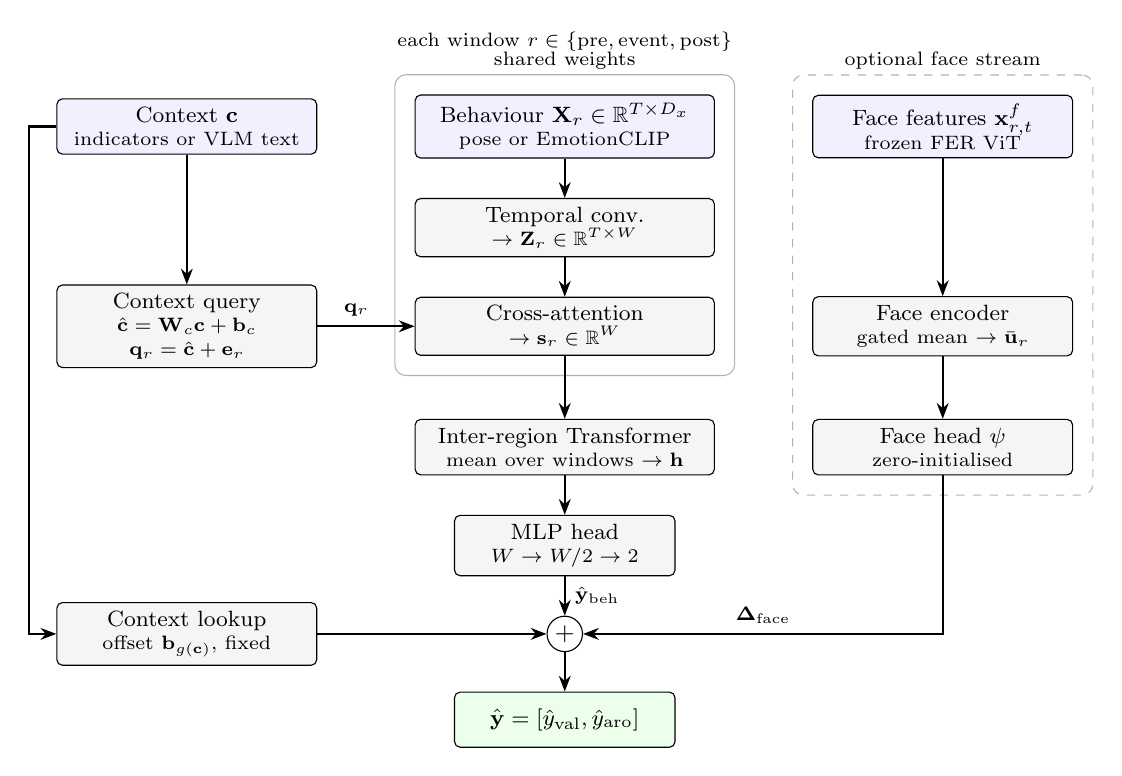
\begin{tikzpicture}[node distance=5mm]
  % Behaviour stream for one window r; the frame marks modules shared by the three windows
  \node[inp,minimum width=3.8cm] (X) {Behaviour $\mX_r\in\R^{T\times D_x}$\\[-1pt]{\scriptsize pose or EmotionCLIP}};
  \node[op,minimum width=3.8cm,below=of X] (T) {Temporal conv.\\[-1pt]{\scriptsize $\to\mZ_r\in\R^{T\times W}$}};
  \node[op,minimum width=3.8cm,below=of T] (A) {Cross-attention\\[-1pt]{\scriptsize $\to\vs_r\in\R^{W}$}};
  \begin{scope}[on background layer]
    \node[winframe,fit=(X)(T)(A)] (win) {};
  \end{scope}
  \node[framelabel,anchor=south] at (win.north) {each window $r\in\{\text{pre},\text{event},\text{post}\}$\\[-1pt]shared weights};
  \draw[arr] (X) -- (T);
  \draw[arr] (T) -- (A);

  % Fusion and output
  \node[op,minimum width=3.8cm,below=8mm of A] (RT) {Inter-region Transformer\\[-1pt]{\scriptsize mean over windows $\to\vh$}};
  \node[op,minimum width=2.8cm,below=of RT] (H) {MLP head\\[-1pt]{\scriptsize $W\to W/2\to 2$}};
  \node[draw,circle,inner sep=0pt,minimum size=4.5mm,font=\small,below=of H] (plus) {$+$};
  \node[outputnode,minimum width=2.8cm,below=of plus] (Y) {$\vy=[\hat y_{\text{val}},\hat y_{\text{aro}}]$};
  \draw[arr] (A) -- (RT);
  \draw[arr] (RT) -- (H);
  \draw[arr] (H) -- node[right,font=\scriptsize]{$\vy_{\text{beh}}$} (plus);
  \draw[arr] (plus) -- (Y);

  % Context: query for the cross-attention, and key for the fixed lookup offset
  \node[inp,minimum width=3.3cm] (C) at ($(X)+(-4.8,0)$) {Context $\vc$\\[-1pt]{\scriptsize indicators or VLM text}};
  \node[op,minimum width=3.3cm] (Q) at (C |- A) {Context query\\[-1pt]{\scriptsize $\vchat=\mW_c\vc+\vb_c$}\\[-1pt]{\scriptsize $\vq_r=\vchat+\ve_r$}};
  \node[op,minimum width=3.3cm] (Lk) at (C |- plus) {Context lookup\\[-1pt]{\scriptsize offset $\vb_{g(\vc)}$, fixed}};
  \draw[arr] (C) -- (Q);
  \draw[arr] (Q.east) -- node[pos=0.4,above,font=\scriptsize]{$\vq_r$} (Q.east -| A.west);
  \draw[arr] (C.west) -- ++(-3.5mm,0) |- (Lk.west);
  \draw[arr] (Lk.east) -- (plus.west);

  % Optional face stream
  \node[inp,minimum width=3.3cm] (F) at ($(X)+(4.8,0)$) {Face features $\mathbf{x}^{f}_{r,t}$\\[-1pt]{\scriptsize frozen FER ViT}};
  \node[op,minimum width=3.3cm] (FE) at (F |- A) {Face encoder\\[-1pt]{\scriptsize gated mean $\to\bar{\vu}_r$}};
  \node[op,minimum width=3.3cm] (FH) at (F |- RT) {Face head $\psi$\\[-1pt]{\scriptsize zero-initialised}};
  \begin{scope}[on background layer]
    \node[faceframe,fit=(F)(FE)(FH)] (face) {};
  \end{scope}
  \node[framelabel,anchor=south] at (face.north) {optional face stream};
  \draw[arr] (F) -- (FE);
  \draw[arr] (FE) -- (FH);
  \draw[arr] (FH.south) |- node[pos=0.75,above,font=\scriptsize]{$\bm{\Delta}_{\text{face}}$} (plus.east);
\end{tikzpicture}
\caption{ContextPose. Each window's behaviour sequence (pose features or subject-aware EmotionCLIP embeddings) is encoded by a temporal convolution and summarised by cross-attention, with a query formed from the projected context and a learned region embedding. The framed modules share their weights across the three windows. A Transformer layer relates the three window summaries, which are averaged and decoded to valence and arousal. The output is a residual on a fixed context-lookup offset, and the optional face stream (dashed) adds a zero-initialised correction.}
\label{fig:arch}
\end{figure}
%-----------------------------------------------------------------------------

\subsection{Problem formulation and inputs}
\label{sec:inputs}

We organise each clip into three event-centred intervals, indexed by $r\in\regions=\{\text{pre},\text{event},\text{post}\}$: a 5\,s pre-event interval, the event interval itself, and a 5\,s post-event interval. Clips lasting 10\,s or less are omitted because they contain no event frames under this partition. Each interval is resampled to $T=32$ temporal steps, and its behaviour input is a sequence of step vectors $\mX_r\in\R^{T\times D_x}$, built either from pose or from EmotionCLIP as described below. The overall clip is associated with an event-context vector $\vc\in\R^{d_c}$. If the facial branch is active, each interval additionally provides face embeddings $\mathbf{X}^f_r\in\R^{T\times D}$ and a binary validity mask $\mathbf{m}_r\in\{0,1\}^{T}$. The network outputs two unconstrained values $\vy\in\R^2$, corresponding to valence and arousal, whose interpretation is specified by the selected learning objective.

% \paragraph{Pose representation.}
 % \We retain $J=11$ upper-body COCO landmarks, comprising the nose, eyes, ears, shoulders, elbows, and wrists, extracted at $f_s=25$\,fps. Let $\mathbf{p}_{n,j}\in\R^2$ denote the image coordinates of joint $j$ in frame $n$. To reduce sensitivity to camera placement and apparent subject scale, coordinates are centred at the shoulder midpoint $\mathbf{o}_n$ and normalised by the clip-level median shoulder width $w$:

% \begin{equation}
%   \tilde{\mathbf{p}}_{n,j} = \frac{\mathbf{p}_{n,j}-\mathbf{o}_n}{w},
% \end{equation}

% This transformation suppresses differences in image position and apparent camera distance while retaining relative body configuration. To obtain fixed-size inputs from intervals of unequal duration, we resample each interval to $T=32$ temporal steps. Each joint is described by $F=4$ features: two normalised coordinates, detector confidence restricted to $[0,1]$, and movement speed. Missing detections are assigned zero coordinates and confidence. During interpolation, a step uses its two surrounding observations when both exist; if only one exists, that observation is retained, and if neither exists, the step remains zero. This avoids inventing trajectories across missing observations, with the confidence feature explicitly indicating uncertainty.

% Fixed-length resampling alone does not preserve movement rate: an event lasting 20\,s and a surrounding interval lasting 5\,s would both contain 32 steps despite their different physical durations. We therefore calculate joint speed from the original frame sequence, before temporal resampling, and express it in shoulder widths per second:

% \begin{equation}
%   v_{n,j} = \min\!\left(f_s\,\lVert\tilde{\mathbf{p}}_{n,j}-\tilde{\mathbf{p}}_{n-1,j}\rVert_2,\; v_{\max}\right), \qquad v_{\max}=20.
% \end{equation}

% If a valid previous observation is unavailable, the next observed frame is used; joints lacking a valid neighbouring observation receive zero speed. The limit $v_{\max}$ reduces sensitivity to abrupt tracking errors. For each resampled step, the speed feature is the average over observed frames in a centred span of approximately $N_r/T$ original frames, where $N_r$ is the interval length. Accordingly, the feature retains a consistent real-time interpretation across intervals.

\paragraph{Pose input.}


\paragraph{Subject-aware video input.} Alternatively, each step is described directly from the video by EmotionCLIP (Zhang et al., 2023), a CLIP ViT-B/32 image encoder trained on vlog videos and their transcripts to represent the emotional state of a designated person. EmotionCLIP is subject-aware: alongside the RGB frame, it receives a binary mask marking the person to be read, which is average-pooled over each $32\times32$ patch and added to that patch's positional embedding. The encoder therefore attends to the subject's body and face while still seeing the surrounding scene. At each of the $T$ steps, we take the corresponding video frame, crop a square centred on the child with side 0.875 times the frame's shorter side, and resize it to 224\,px with ImageNet normalisation. EmotionCLIP was trained with person boxes from an object detector; we instead build the mask from the child's tracked joints, as their bounding box padded by 0.3 shoulder widths and extended downwards, because the 11 joints cover mainly the upper body. Deriving the mask from the child's own track keeps it on the child rather than on an adult or a person shown on a screen. When the child is not tracked within two frames of the step, the mask is left empty rather than guessed. The frozen encoder's output is $\ell_2$-normalised to a 512-dimensional frame embedding, and a binary flag recording whether the child was tracked is appended, giving $D_x=513$. Like the confidence feature of the pose input, this flag tells the encoder which steps are less reliable. We use EmotionCLIP's per-frame encoder rather than its own temporal Transformer, so that our temporal encoder and context-queried attention operate on the same $T$ steps for both inputs. With this input, pose only determines where the crop and mask are placed; joint coordinates do not enter the features.

\subsection{Temporal behaviour encoder}
\label{sec:pose-encoder}

For each region, the behaviour input $\mX_r\in\R^{T\times D_x}$ holds one vector per step: the concatenated joint features for pose, or the flagged frame embedding for EmotionCLIP. Two one-dimensional temporal convolutions turn this sequence into $W$-dimensional tokens:

\begin{equation}
  \mZ_r = \GELU\!\big(\mathrm{Conv}_2(\GELU(\mathrm{Conv}_1(\mX_r)))\big)\in\R^{T\times W}.
\end{equation}

Each convolution has kernel size 3 with zero padding, so every output step is a learned linear function of the input at that step and its two neighbours. $\mathrm{Conv}_1$ maps $D_x$ input channels to $W$, and $\mathrm{Conv}_2$ maps $W$ to $W$. Only $\mathrm{Conv}_1$ depends on the choice of input; every later layer is identical for pose and EmotionCLIP. Stacking the two layers yields a five-step receptive field, enabling each token $\mathbf{z}_{r,t}$ to encode local change across neighbouring steps rather than a single isolated observation. Parameters are shared across the three regions. No explicit temporal positional embedding is introduced: ordering is represented locally through convolution, while the subsequent within-region attention is otherwise permutation-invariant over the generated tokens.

\subsection{Context encoder}
\label{sec:context}

We investigate three alternative representations of environmental context, each providing a different level of semantic detail. The first consists of four annotator-defined binary indicators describing social interaction, auditory events, activity or object changes, and visual or media events ($d_c=4$); clips without annotated events receive an all-zero vector. The second expresses these indicators as natural-language event descriptions and encodes the sentences using a frozen CLIP ViT-L/14 text encoder, followed by $\ell_2$ normalisation ($d_c=768$). As this text is generated from the event indicators, it does not add independent scene content; only nine unique sentences occur in the development clips. The third representation instead derives descriptions from the video itself. Qwen3-Omni generates accounts of the scene, the child's behaviour, and audible surroundings over successive 5--6\,s segments. These descriptions are encoded using all-MiniLM-L6-v2, averaged across segments, and $\ell_2$-normalised to obtain a clip-level vector ($d_c=384$). Each representation is mapped to the common latent width using a linear projection:

\begin{equation}
  \vchat = \mW_c\,\vc + \vb_c\in\R^{W}.
\end{equation}

In addition, each temporal region is assigned a learned embedding $\ve_r\in\R^W$, with parameters initialised from $\mathcal{N}(0,0.02^2)$. Because the cross-attention module shares parameters across regions, these embeddings provide the region-specific identity needed to distinguish pre-event, event, and post-event queries.

\subsection{Context-queried temporal attention}
\label{sec:cross-attention}

The central fusion mechanism is context-conditioned temporal cross-attention. For each region, the model constructs a single query from the projected environmental context and the corresponding region embedding, $\vq_r = \vchat + \ve_r$; keys and values come exclusively from that region's behaviour tokens. For one attention head, the weights over the $T$ steps and the resulting summary are

\begin{equation}
  \begin{aligned}
    \bm{\alpha}_r &= \softmax\!\left(\frac{(\vq_r\mW^{Q})(\mZ_r\mW^{K})^{\top}}{\sqrt{d_h}}\right)\in\R^{T},\\
    \vs_r &= \sum_{t=1}^{T}\alpha_{r,t}\,\mathbf{z}_{r,t}\mW^{V}.
  \end{aligned}
  \label{eq:attn}
\end{equation}

We use $H=4$ heads, each with its own projections $\mW^{Q},\mW^{K},\mW^{V}\in\R^{W\times d_h}$ and width $d_h=W/H$. The head outputs are concatenated and mixed by an output projection $\mW^{O}\in\R^{W\times W}$ to give $\vs_r\in\R^{W}$; biases are omitted from the notation. The same attention projections are reused across all three regions.

As shown by Equation~\eqref{eq:attn}, environmental context influences the attention distribution rather than being inserted directly into the behaviour-derived values. For each head, the region summary is a weighted average of projected behaviour tokens, and the context vector $\vc$ affects which tokens receive the greatest weights. Consequently, an auditory event and a social interaction may lead the model to emphasise different periods of the same behavioural sequence. This mechanism produces a fixed-dimensional summary $\vs_r$ for every region, independent of its original temporal extent.

\subsection{Inter-region Transformer and prediction head}
\label{sec:region-transformer}

The regional summaries are assembled into $\mS=[\vs_{\text{pre}};\vs_{\text{event}};\vs_{\text{post}}]\in\R^{3\times W}$. A single post-normalisation Transformer encoder layer models relationships among these representations:

\begin{equation}
  \mS' = \LN\big(\mS + \mathrm{MHSA}(\mS)\big),
  \qquad
  \mS'' = \LN\big(\mS' + \mathrm{FFN}(\mS')\big).
\end{equation}

Here $\mathrm{MHSA}$ is self-attention over the three region vectors with $H=4$ heads, and $\mathrm{FFN}$ is a two-layer network of width $2W$ with a ReLU activation. Dropout, omitted from the equation, is applied to the attention weights, inside the feed-forward network, and to the output of each sublayer. Through this operation, the representation of a given region can incorporate information from the others. For example, behaviour during the event can be interpreted in relation to the child's behaviour immediately before and afterward. We obtain a clip-level representation by averaging the transformed regional outputs:

\begin{equation}
  \vh = \frac{1}{3}\sum_{r\in\regions}\mS''_r\in\R^{W}.
\end{equation}

We do not apply positional encodings at this stage. Since self-attention followed by mean aggregation is invariant to permutations of the three input rows, the ordering of the regional vectors is not explicitly available to the final representation. The learned region embeddings introduced at the preceding attention stage are therefore the only source of region identity.

An optional \emph{context skip} connection modifies the fused representation as $\vh\leftarrow\vh+\vchat$, allowing context to influence the output directly as well as through temporal selection. A two-layer MLP with an intermediate dimension of $W/2$ maps the resulting representation to the behaviour-branch valence and arousal scores:

\begin{equation}
  \vy_{\text{beh}} = \mathrm{MLP}(\vh) = \mW_4\,\GELU(\mW_3\vh+\vb_3)+\vb_4\in\R^{2},
\end{equation}

with dropout of rate $p_h$ applied to its input during training.

\subsection{Gated face stream}
\label{sec:face}

Although facial expression can provide strong evidence of valence, its reliability varies considerably in naturalistic recordings of children. Face crops may be occluded, blurred, poorly illuminated, or affected by head rotation. We therefore model facial information through a separate auxiliary branch that contributes an additive correction to the behaviour-based estimate only when adequate facial observations are available.

For each of the $T$ temporal positions in a region, we extract the face crop from the nearest video frame. The crop is centred using the tracked facial landmarks, covers a square region of width 0.9 shoulder widths, and is resized to 224\,px. A frozen facial-expression ViT pretrained on FER2013 produces a $D=768$-dimensional [CLS] embedding $\mathbf{x}^f_{r,t}\in\R^{D}$. A binary mask $m_{r,t}$ identifies valid crops according to three criteria: (i) the pose tracker detects the nose and both eyes, indicating a frontal face; (ii) YuNet independently detects a face at that location with confidence at least 0.8; and (iii) the crop exceeds a mean grey-level threshold of 40 and a Laplacian-variance threshold of 10. These checks reject unreliable detections, including cases in which the pose estimator reports facial landmarks despite occlusion or a lowered head. Invalid steps have their features set to zero.

Each face embedding is projected to 32 dimensions, and the valid steps of each region are averaged:

\begin{equation}
  \begin{aligned}
    \vu_{r,t} &= \GELU\big(\mW_f\,\LN(\mathbf{x}^f_{r,t})+\vb_f\big)\in\R^{32},\\
    \bar{\vu}_r &= \frac{\sum_{t} m_{r,t}\,\vu_{r,t}}{\max\big(1,\sum_{t} m_{r,t}\big)}.
  \end{aligned}
\end{equation}

The denominator $\max(1,\cdot)$ ensures that a region with no valid facial frames has a zero summary. The three region summaries are concatenated and passed to a two-layer head $\psi$ ($96\to W/2\to k$) with input dropout $p_h$, which produces the correction

\begin{equation}
  \bm{\Delta}_{\text{face}} =
  \begin{cases}
    \psi\big([\bar{\vu}_{\text{pre}};\bar{\vu}_{\text{event}};\bar{\vu}_{\text{post}}]\big), & \text{if } \sum_{r,t} m_{r,t}>0,\\
    \mathbf{0}, & \text{otherwise}.
  \end{cases}
  \label{eq:face}
\end{equation}

With $k=2$, the face stream corrects both valence and arousal; with $k=1$, it corrects valence only and the arousal entry of $\bm{\Delta}_{\text{face}}$ is zero.

We introduce three safeguards to limit the effect of low-quality facial information. First, the final layer of $\psi$ is initialised to zero, so the model initially reproduces the behaviour-and-context prediction and only later learns an additional facial contribution. Second, the second case of Equation~\eqref{eq:face} forces $\bm{\Delta}_{\text{face}}=\mathbf{0}$ when no valid facial step exists anywhere in the clip, preventing a spurious correction from the head's bias. Third, during training, the complete face branch is randomly removed with probability $p_f$ by setting every mask entry $m_{r,t}$ of the clip to zero. This face dropout also makes the correction zero and encourages the remaining modalities to support the prediction independently.

\subsection{Residual prediction on a context lookup}
\label{sec:residual}

Because event-indicator combinations are informative about the observed annotation distribution, a simple context-conditioned lookup provides a useful baseline. Given the small development sample of approximately 150 clips, we train ContextPose to estimate deviations from this baseline rather than requiring its neural branches to learn the full prediction directly:

\begin{equation}
  \vy = \vy_{\text{beh}} + \bm{\Delta}_{\text{face}} + \vb_{g(\vc)}.
  \label{eq:output}
\end{equation}

In Equation~\eqref{eq:output}, $g(\vc)$ identifies the event-indicator combination associated with the clip, and $\vb_{g}\in\R^2$ denotes its fixed baseline offset. Offsets are estimated exclusively from training examples within each cross-validation fold and are not updated by gradient descent, thereby excluding evaluation data from baseline estimation. For vote-based learning, each offset equals the log-odds of the group's mean vote proportion $\bar{\pi}_{g}$. We clip this proportion to $[\epsilon,1-\epsilon]$, where $\epsilon=0.02$, to avoid infinite log-odds:

\begin{equation}
  \vb_{g} = \log\frac{\bar{\pi}_{g}}{1-\bar{\pi}_{g}}.
\end{equation}

For regression, the offset is instead the median target value for the corresponding group. If fewer than three training clips are available for a group, the global training-set estimate is used. Disabling the lookup sets the offset to zero; the prediction head's bias then supplies any learned constant component, and no label statistics are injected through this branch.

\subsection{Output parameterisation and objective}
\label{sec:objective}

Three annotators assessed each clip, assigning positive, neutral, or negative valence and either high or low arousal. Given the moderate inter-annotator agreement, our primary objective retains the distribution of votes instead of collapsing them to a single consensus class. For each dimension, $\pi\in[0,1]$ denotes the proportion of known votes for positive valence or high arousal. The prediction $\hat{y}$ is interpreted as the logit of that vote probability, and training minimises binary cross-entropy with the soft vote proportion for both outputs, averaged over the batch:

\begin{equation}
  \mathcal{L} = -\sum_{k\in\{\text{val},\text{aro}\}}\Big[\pi_k\log\sigma(\hat{y}_k)+(1-\pi_k)\log\big(1-\sigma(\hat{y}_k)\big)\Big].
\end{equation}

During inference, $\sigma(\hat{y}_k)$ gives the estimated vote probability, used to distinguish positive from non-positive valence or high from low arousal after applying a threshold. Thresholds are chosen to maximise balanced accuracy using only model-fitting and selection data, never evaluation clips. For the alternative regression objective, the two outputs represent consensus valence and arousal directly and are optimised using mean squared error.

\subsection{Stream ablations}
\label{sec:ablations}

To assess the contribution of each modality, we evaluate stream-removal variants that retain the same basic prediction framework while disabling selected inputs:

\begin{align}
  \text{behaviour only:}\quad & \vy = \vy_{\text{beh}}\big|_{\vchat=\mathbf{0}} + \bm{\Delta}_{\text{face}} + \vb, \\
  \text{context only:}\quad & \vy = \mathrm{MLP}(\vchat) + \bm{\Delta}_{\text{face}} + \vb, \\
  \text{face only:}\quad & \vy = \bm{\Delta}_{\text{face}} + \vb.
\end{align}

In the behaviour-only variant, the projected context is set to zero, leaving the learned region embeddings to provide the cross-attention queries; it can be run with either pose or EmotionCLIP input. In the context-only variant, the behaviour pathway is bypassed and the prediction MLP operates directly on the projected context. The face-only configuration removes the behaviour prediction and retains the facial correction where that branch is enabled. Across these experiments, $\vb$ denotes either the fixed context-dependent offset $\vb_{g(\vc)}$ or zero when the lookup is inactive. Thus, when the lookup is enabled, the nominal face-only condition still incorporates event information through its baseline offset.

\subsection{Implementation details}
\label{sec:impl}

We keep the network compact to limit overfitting on the development set of approximately 150 clips. Table~\ref{tab:hparams} summarises the architectural and optimisation settings. With latent width $W=64$, pose input, and the indicator context, the model contains 73.6k trainable parameters; using VLM or CLIP features increases this to 98.0k and 122.5k, respectively, primarily due to the input projection. Replacing pose with EmotionCLIP input raises the indicator-context model to 163.7k parameters, entirely through the first convolution, whose input grows from 44 to 513 channels; the frozen EmotionCLIP encoder itself is not trained. The optional face branch introduces another 29.3k parameters, largely from mapping the 768-dimensional face embedding to 32 dimensions.

We optimise all variants using AdamW with learning rate $3\times10^{-4}$, weight decay 0.05, and batch size 16. Training lasts at most 60 epochs for indicator and CLIP contexts or 150 epochs for VLM context, with early stopping after 10 epochs without validation improvement. The selected checkpoint minimises validation cross-entropy in the vote-prediction setting and validation mean absolute error in regression. To augment each training pose sequence, we apply random rotations within $\pm15^\circ$, scale factors in $[0.9,1.1]$, and Gaussian coordinate noise of standard deviation $\sigma=0.02$ shoulder widths. Horizontal reflection is applied with probability 0.5, reversing the horizontal coordinate and exchanging left and right joints. All regions of a clip receive the same transform, and missing joints remain unchanged. These transforms act on joint coordinates, so they apply only to pose input; EmotionCLIP embeddings are extracted once from fixed crops and used without augmentation. For final evaluation, we ensemble five independently seeded models, averaging their prediction scores and using a majority vote of their binary decisions.

\begin{table}[t]
\centering
\caption{Hyper-parameters of ContextPose. Parameter counts use indicator context.}
\label{tab:hparams}
\footnotesize
\setlength{\tabcolsep}{4pt}
\begin{tabular}{@{}lr@{}}
\toprule
Hyper-parameter & Value \\
\midrule
Steps per window $T$ / joints $J$ / features $F$ & 32 / 11 / 4 \\
Behaviour input $D_x$ (pose / EmotionCLIP) & 44 / 513 \\
Context $d_c$ (indicators / CLIP / VLM) & 4 / 768 / 384 \\
Conv.\ layers / kernel / activation & 2 / 3 / GELU \\
Model width $W$ & 64 \\
Attention heads $H$ / head width $d_h$ & 4 / 16 \\
Region Transformer layers / heads / FFN & 1 / 4 / $2W$ \\
Face input $D$ / encoding width & 768 / 32 \\
Prediction head hidden width & $W/2$ \\
Dropout: Transformer, head $p_h$, face $p_f$ & 0.3 \\
\midrule
Optimiser & AdamW \\
Learning rate / weight decay & $3{\times}10^{-4}$ / 0.05 \\
Batch size / max.\ epochs / patience & 16 / 60 / 10 \\
Ensemble size (seeds) & 5 \\
\midrule
Parameters, pose (no face / face) & 73.6k / 102.9k \\
Parameters, EmotionCLIP (no face / face) & 163.7k / 193.0k \\
\bottomrule
\end{tabular}
\end{table}

\end{document}
